\documentclass{article}
\usepackage{graphicx}
\usepackage[margin=1.5cm]{geometry}
\usepackage{amsmath}

\begin{document}

\title{Thursday Reading Assessment: Chapter 2-1 through 2-7}
\author{Prof. Jordan C. Hanson}

\maketitle

\section{Binary and Other Number Systems}

\begin{enumerate}
\item What is the \textit{weight} of the digit 6 in each of the following numbers? (a) 1386 (b) 54,692 (c) 671,920 \\ \vspace{0.2cm}
\item Convert each number to scientific notation: (a) 1400 (b) 0.000071 (c) 130,000,000 (d) 1/3 \\ \vspace{0.2cm}
\item What is the largest number you could represent with three \textit{decimal} digits?
\item What is the largest number you could represent with three \textit{binary} digits?
\item Decode the following into decimal: (a) 1111 (b) 11110000 (c) 1111 0000 0000 \\ \vspace{0.2cm}
\end{enumerate}

\section{Binary Addition and Signed Numbers}

\begin{figure}[hb]
\centering
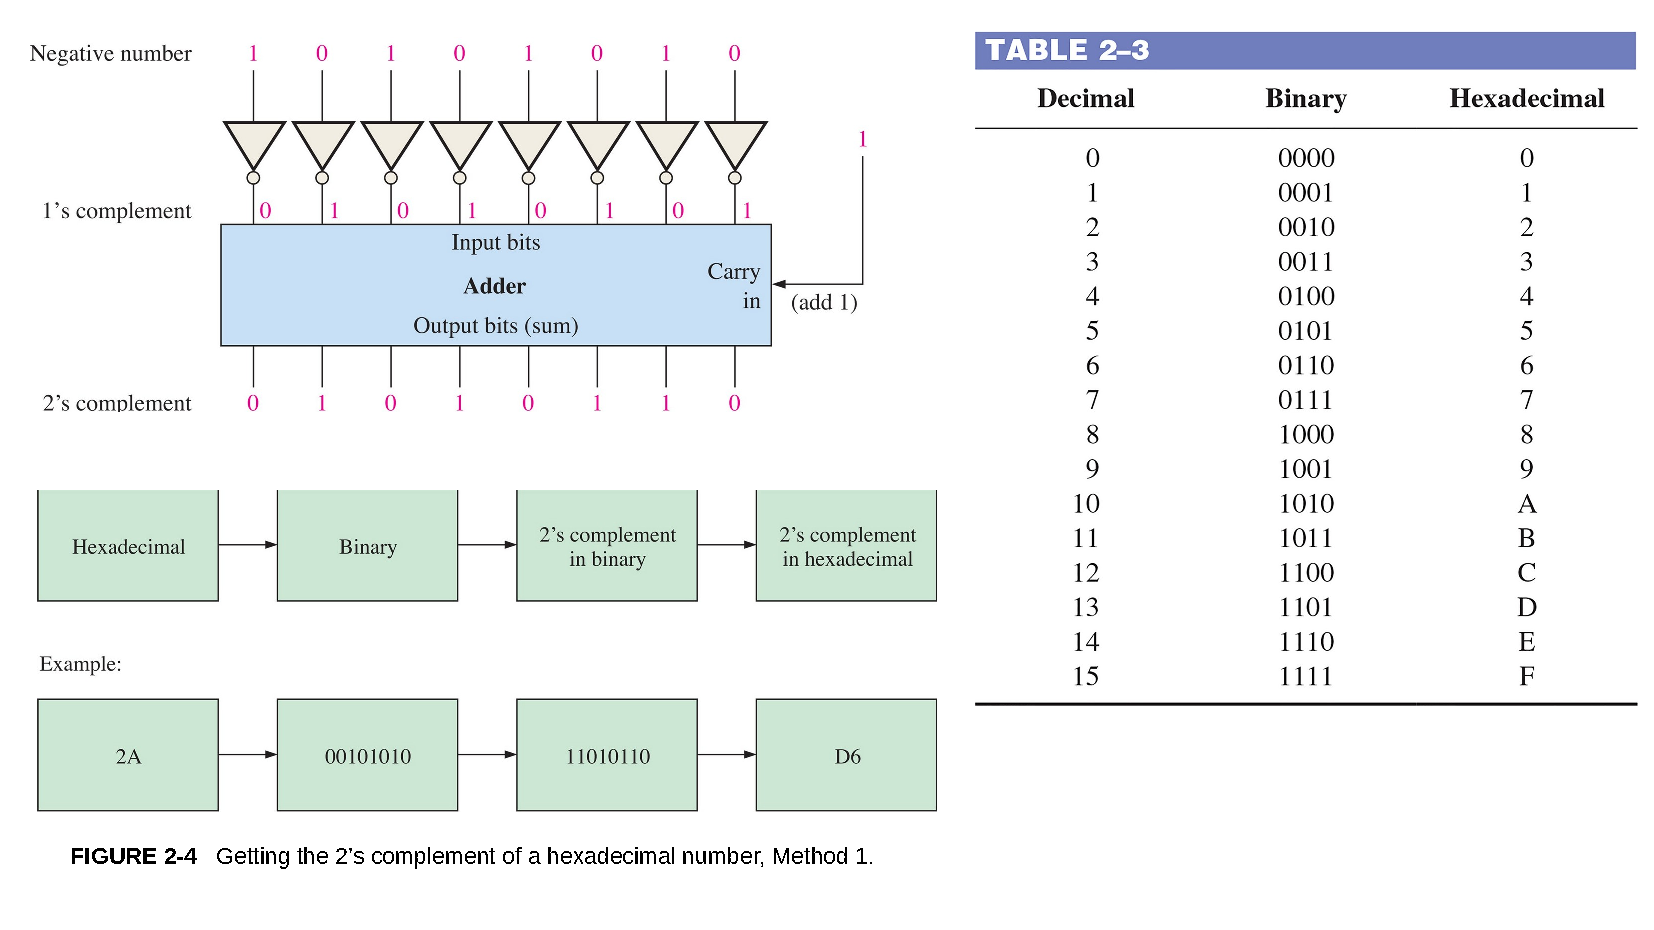
\includegraphics[width=0.45\textwidth,trim=0cm 8cm 12cm 0cm,clip=true]{figures/quiz_graphic.pdf} \hspace{0.25cm}
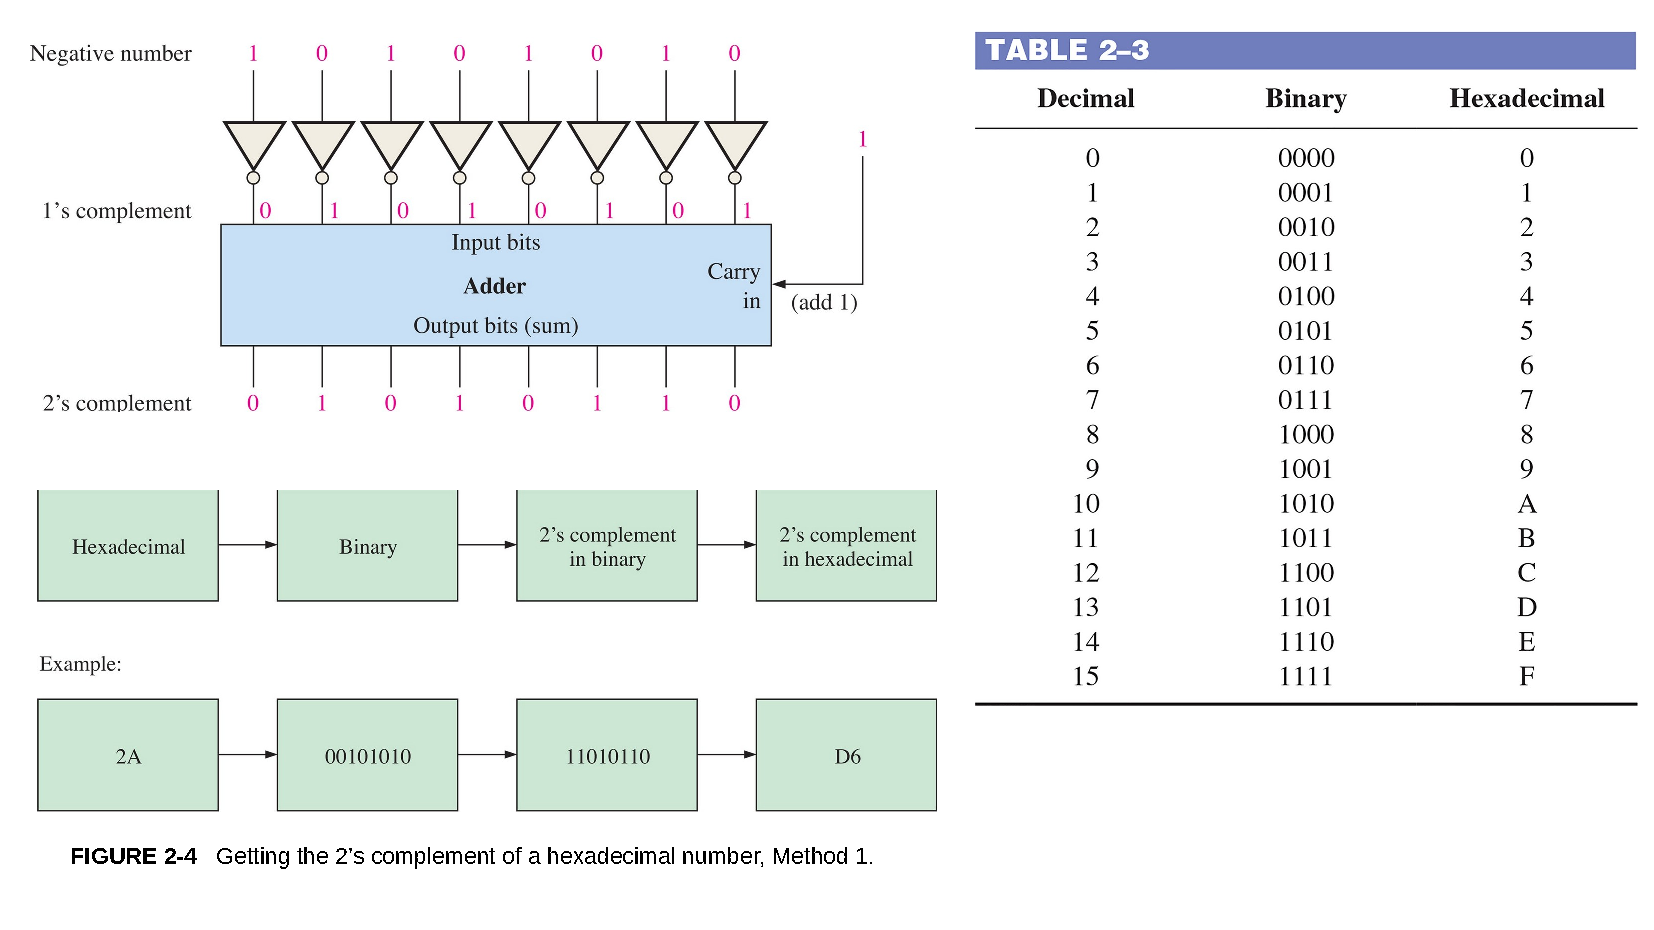
\includegraphics[width=0.35\textwidth,trim=16cm 7cm 0cm 0cm,clip=true]{figures/quiz_graphic.pdf}
\caption{\label{fig:quiz}(Top left) a circuit used in binary conversion. (Top right) Decimal, binary, and hexadecimal digits. (Bottom left) A procedure for hexadecimal conversion.}
\end{figure}

\begin{enumerate}
\item What is the purpose of the circuit in Fig. \ref{fig:quiz} (left)? \textit{Hint: try adding the input to the output.}
\item Using Fig. \ref{fig:quiz} (right), what is 256 in binary and hexadecimal?
\item What is -127 in binary and hexadecimal?
\end{enumerate}

\end{document}
